\section{Random Variables}
\subsection{Random variables}
\begin{bdef}{Random variables}\label{randomvariables}
    When an experiment is performed, we are often more interested in a function of the outcome as opposed to the actual outcome itself. For instance, when tossing a handful of dice, we may care more about the sum of the numbers rolled than the separate values of each die, or when flipping coins, we may care more about the total number of heads flipped than the actual sequence of flips.

    These quantities of interest -- more formally, these functions from $S$ to $\Real$ -- are known as \textbf{random variables}. Because the value of a random variable is determined by the outcome of the experiment, we may assign probabilities to the possible values of the random variable.
\end{bdef}
\begin{changebar}
    \begin{example}
        Suppose our experiment consists of tossing 3 fair coins. If we let $Y$ denote the number of heads that appear, then $Y$ is a random variable with range $\left\{ 0, 1, 2, 3 \right\}$ and respective probabilities \[
            \begin{aligned}
                P\left\{ Y = 0 \right\} &= P(\left\{ (T, T, T) \right\}) &= \frac{1}{8} \\
                P\left\{ Y = 1 \right\} &= P(\left\{ (H, T, T), (T, H, T), (T, T, H) \right\}) &= \frac{3}{8} \\
                P\left\{ Y = 2 \right\} &= P(\left\{ (H, H, T), (H, T, H), (T, H, H) \right\}) &= \frac{3}{8} \\
                P\left\{ Y = 3 \right\} &= P(\left\{ (H, H, H) \right\}) &= \frac{1}{8}
            \end{aligned}    
        \]
        We also have \[
            1 = P\left( \bigcup^3_{i = 0} \left\{ Y = i \right\} \right) = \sum^3_{i = 0} P\left\{ Y = i \right\}    
        \]
    \end{example}
\end{changebar}

\begin{changebar}
    \begin{example}
        Four balls are to be randomly selected, without replacement, from an urn that contains 20 balls numbered 1 through 20. If $X$ is the largest ball selected, then $X$ is a random variable that takes on one of the values $4, 5, \dots, 20$. Because each of the $\displaystyle {20 \choose 4}$ possible selections of $4$ of the $20$ balls is equally likely, the probability that $X$ takes on each of its possible values is \[
            P\left\{ X = i \right\}\frac{{i - 1 \choose 3}}{{20 \choose 4}},\: i = 4, \dots, 20.    
        \] This is because the number of selections that result in $X = i$ is the number of selections that result in the ball numbered $i$ and three of the balls numbered $1$ through $i - 3$ being selected. As there are $\displaystyle {1 \choose 1}{i - 1 \choose 3}$ such selections, the preceding follows.
    \end{example}
\end{changebar}

\begin{changebar}
    \begin{example}
        Independent trials consisting of the flipping of a coin having probability $p$ of coming up heads are continually performed until either a head occurs or a total of $n$ flips is made. If we let $X$ denote the number of times the coin is flipped, then $X$ is a random variable taking on one of the values $1, 2, 3, \dots, n$, with respective probabilities \[
            \begin{aligned}
                P\left\{ X = 1 \right\} &= P\left\{ (h) \right\} &=& p \\
                P\left\{ X = 2 \right\} &= P\left\{ (t, h) \right\} &=& (1-p)p \\
                P\left\{ X = 3 \right\} &= P\left\{ (t, t, h) \right\} &=& (1-p)^2p \\
                \vdots && \vdots & \\
                P\left\{ X = n - 1 \right\} &= P\left\{ (\underbrace{t, t, \dots, t}_{n - 2}, h) \right\} &=& (1-p)^{n-2}p \\
                P\left\{ X = n \right\} &= P\left\{ (\underbrace{t, t, \dots, t}_{n - 1}, t), (\underbrace{t, t, \dots, t}_{n - 1}, h) \right\} &=& (1-p)^{n-1}
            \end{aligned}    
        \]
    \end{example}    
\end{changebar}
\begin{bdef}{Distribution function}\label{distributionfunction}
    For a random variable $X$, the function $F: \Real \to [0, 1]$ defined by \[
        F(x) = P\left\{ X \leq x \right\}
    \] is called the \textbf{cumulative distribution function}, or more simply, the \textbf{distribution function} of $X$. Thus, the distribution function specifies, for all real values $x$, the probability that the random variable is less than or equal to $x$.
    
    Suppose that $a \leq b$. Then, because the event $\left\{ X \leq a \right\}$ is contained in the event $\left\{ X \leq b \right\}$, it follows that $F(a) \leq F(b)$. In other words, $F(x)$ is a nondecreasing function of $x$. Other properties of $F$ are given in \autoref{cumdistproperties}.
\end{bdef}
\pagebreak
\subsection{Discrete random variables}
\begin{bdef}{Discrete random variables}\label{discreterandomvariables}
    A random variable that can take on at most a countable number of possible values is said to be \textbf{discrete}.
\end{bdef}
\begin{bdef}{Probability mass function}\label{probabilitymassfunction}
    For a discrete random variable $X$, we define the \textbf{probability mass function} $p(a)$ of $X$ by \[
        p(a) = P\left\{ X = a \right\}.    
    \] $p(a)$ is positive for at most a countable number of values of $a$. That is, if $X$ must assume one of the values $x_1, x_2, \dots, x_n$, then \[
        \begin{cases}
            p(x_i) \geq 0 & \text{for } i = 1, 2, \dots \\
            p(x) = 0 & \text{otherwise} 
        \end{cases}    
    \] Since $X$ must take one of the values $x_i$, we have \[
        \sum^\infty_{i = 1} p(x_i) = 1.    
    \]
\end{bdef}
It is often instructive to plot the probability mass function by plotting $x_i$ on the $x$-axis against $p(x_i)$ on the $y$-axis. For example, the graph of the probability mass function of the random variable representing the sum of two dice would look like:
\begin{center}    
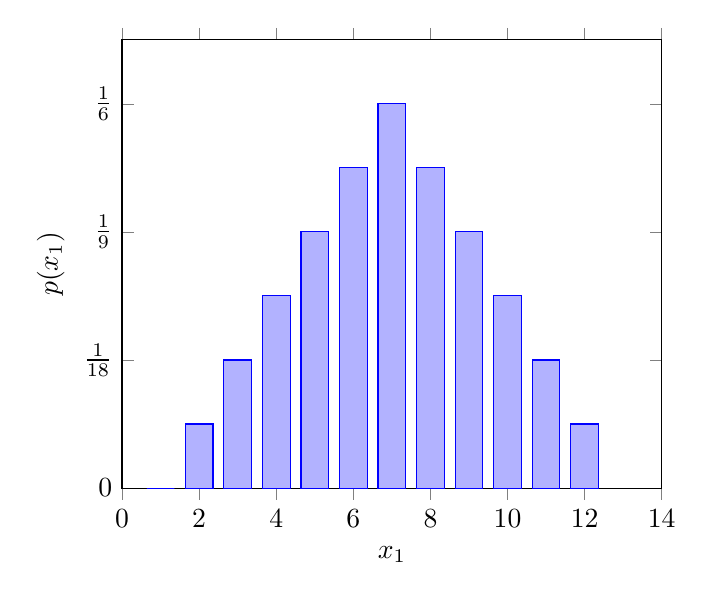
\begin{tikzpicture}
    \begin{axis}[
        ybar, 
        xmin = 0, 
        xmax = 14, 
        ymin = 0, 
        ymax = 7/36,
        yticklabel style={/pgf/number format/frac, /pgf/number format/frac shift=2}, 
        ytick={0, 2/36, 4/36, 6/36},
        xlabel={$x_1$}, 
        ylabel={$p(x_1)$}]
        \addplot coordinates {
            (1, 0)
            (2, 1/36)
            (3, 2/36)
            (4, 3/36)
            (5, 4/36)
            (6, 5/36)
            (7, 6/36)
            (8, 5/36)
            (9, 4/36)
            (10, 3/36)
            (11, 2/36)
            (12, 1/36)
        };
    \end{axis} 
\end{tikzpicture}
\end{center}
\begin{changebar}
    \begin{example}
        The probability mass function of a random variable $X$ is given by $p(i) = c\lambda^i/i!$, $i = 0, 1, \dots,$ where $\lambda$ is some positive value. Find \begin{enumerate}[label=(\alph*)]
            \item $P\left\{ X = 0 \right\}$.
            \item $P\left\{ X > 2 \right\}$.
        \end{enumerate}
    \end{example}
    \begin{solution}
        Since $\displaystyle \sum^\infty_{i = 0} p(i) = 1$, we have \[
            c \sum^\infty_{i = 0} \frac{\lambda^i}{i!} = 1.    
        \] Because $\displaystyle e^x = \sum^\infty_{i = 0} \frac{x^i}{i!}$, this implies that \[
            ce^\lambda = 1 \text{ or } c = e^{-\lambda}.    
        \]
        Thus, we have: \begin{enumerate}[label=(\alph*)]
            \item $P\left\{ X = 0 \right\} = p(0) = e^{-\lambda}\lambda^0/0! = e^{-\lambda}$
            \item \[
                \begin{aligned}
                    P\left\{ X > 2 \right\} &= 1 - P\left\{ X \leq 2 \right\} \\
                    &= 1 - P\left\{ X = 0 \right\} - P\left\{ X = 1 \right\} - P\left\{ X = 2 \right\} \\
                    &= 1 - e^{-\lambda} - \lambda e^{-\lambda} - \frac{\lambda^2e^{-\lambda}}{2}.
                \end{aligned}    
            \]
        \end{enumerate}
    \end{solution}
\end{changebar}

\pagebreak
\subsection{Properties of the cumulative distribution function}\label{cumdistproperties}